\documentclass[12pt]{report}
\usepackage{graphicx}
\graphicspath{{images/}}
\usepackage{float}
\usepackage{geometry}
\geometry{a4paper, margin=1in}

\usepackage[utf8]{inputenc}
\usepackage[T1]{fontenc}
\usepackage{amsmath}
\usepackage{booktabs}
\usepackage{tabularx}
\usepackage{titlesec}
\titleformat{\chapter}[hang]{\normalfont\Huge\bfseries}{\thechapter.}{1em}{}

\usepackage{setspace}
\usepackage{url}
\usepackage{hyperref}
\hypersetup{colorlinks=true, linkcolor=black, citecolor=black, urlcolor=blue}

\setstretch{1.4}

\begin{document}
\pagenumbering{roman}

\begin{titlepage}
    \begin{center}
        \vspace*{0.4cm}
        {\Large \textbf{Comparison of Lightweight Encryption Algorithms}}\\[0.3cm]

        {\large A comparative study of secure and efficient cryptographic primitives\\
        for resource-constrained embedded systems}\\[1.0cm]

        \textbf{Final Project Report Submitted}\\
        In partial fulfillment of the requirements for the award of the\\
        \textbf{Bachelor of Technology}\\[1.0cm]
        {\large \textbf{Authors}}\\[0.25cm]

        \begin{tabular}{ll}
            \textbf{Rajesh Kumar Jena} & (B122088) \\
            \textbf{Soumil Kumar}      & (B122114) \\
            \textbf{Punit Kumar}       & (B422041)
        \end{tabular}\\[1.0cm]

        {\large \textbf{Under the supervision of}}\\[0.2cm]
        {\textbf{Prof. Debasish Jena}}\\[1.0cm]

        
\includegraphics[width=0.22\textwidth]{iiit-bh-logo.png}\\[0.4cm]
        {\large International Institute of Information Technology, Bhubaneswar}\\[0.15cm]
        {\large May 2026}

    \end{center}
\end{titlepage}

\newpage
\chapter*{Approval of the Viva Voce Board}
\addcontentsline{toc}{chapter}{Approval of the Viva Voce Board}
\vspace{1cm}
\noindent May 19, 2026

\vspace{1cm}

\noindent Certified that the report entitled ``Comparison of Lightweight Encryption Algorithms,''
submitted by Rajesh Kumar Jena (B122088), Soumil Kumar (B122114), and Punit Kumar (B422041)
to the International Institute of Information Technology, Bhubaneswar, in partial fulfillment
of the B.Tech programme requirements for the award of the Bachelor of Technology, has been accepted by the examiners during the viva voce examination held today.

\vfill

\noindent \underline{\hspace{5.5cm}} \hfill \underline{\hspace{5.5cm}}

\noindent Prof. Debasish Jena (Supervisor) \hfill External Examiner

\newpage
\chapter*{Certificate}
\addcontentsline{toc}{chapter}{Certificate}

This is to certify that the report entitled ``Comparison of Lightweight Encryption Algorithms,''
submitted by Rajesh Kumar Jena (B122088), Soumil Kumar (B122114), and Punit Kumar (B422041)
to the International Institute of Information Technology, Bhubaneswar, is a record of bona fide
work carried out under my supervision. The report is submitted for the end-semester evaluation
of the B.Tech programme.

\vfill
\noindent Prof. Debasish Jena

\newpage
\chapter*{Declaration}
\addcontentsline{toc}{chapter}{Declaration}

We hereby declare that:

\begin{enumerate}
    \item The work presented in this report is entirely our own and was carried out under the guidance of our supervisor.
    \item This report has not been submitted, either in part or in full, to any other institution for the award of any degree or diploma.
    \item We have adhered to the Ethical Code of Conduct prescribed by the Institute while carrying out this work.
    \item Wherever we have quoted material from other sources, we have placed such quotations within quotation marks and provided appropriate citations and references.
    \item Whenever we have used ideas, data, analysis, or text derived from other sources, we have duly acknowledged them within the report and included full details in the reference section.
    \item We have followed all guidelines and formatting instructions stipulated by the Institute in the preparation of this report.
\end{enumerate}

\vspace{1cm}

\noindent \textbf{Rajesh Kumar Jena} \hfill \textbf{B122088}\\
\textbf{Soumil Kumar} \hfill \textbf{B122114}\\
\textbf{Punit Kumar} \hfill \textbf{B422041}

\newpage
\chapter*{Acknowledgments}
\addcontentsline{toc}{chapter}{Acknowledgments}

We express our sincere gratitude to our supervisor, Prof.\ Debasish Jena, for his invaluable
guidance, continuous support, and insightful feedback throughout this project. His expertise
was instrumental in helping us navigate challenges and refine our work.

We also thank the faculty and staff of the Department of Computer Science and Engineering and
the Department of Information Technology at the International Institute of Information
Technology, Bhubaneswar, for providing the resources, infrastructure, and academic environment
necessary for the successful completion of this project.

Finally, we extend our heartfelt appreciation to our families and friends for their constant
support and understanding throughout the duration of this work.

\vspace{1cm}

\noindent \textbf{Rajesh Kumar Jena}\\
\textbf{Soumil Kumar}\\
\textbf{Punit Kumar}

\newpage
\chapter*{Abstract}
\addcontentsline{toc}{chapter}{Abstract}

The proliferation of resource-constrained devices in IoT networks, embedded controllers,
and sensor systems has increased the need for lightweight cryptographic solutions.
Conventional encryption algorithms often exceed the computational capabilities, memory
constraints, and energy budgets of such platforms. This study presents a comparative
analysis of three prominent lightweight encryption algorithms---PRESENT, SPECK, and
ASCON---and evaluates their suitability for constrained embedded environments.

The methodology combines theoretical analysis of design principles with empirical
performance benchmarking on a Raspberry Pi Pico microcontroller using Rust
implementations. Metrics, including execution time, memory utilization, and throughput,
are systematically evaluated.

The findings provide a clearer understanding of how lightweight ciphers balance
security and efficiency in practical embedded systems, revealing clear performance
hierarchies with significant variations in throughput, memory footprint, and
security properties that inform practical deployment decisions.

\vspace{1cm}
\noindent \textbf{Keywords}: lightweight cryptography, embedded systems, PRESENT, SPECK,
ASCON, IoT security, performance evaluation, Raspberry Pi Pico, Rust

\newpage
\tableofcontents

\begingroup
\let\clearpage\relax
\listoftables
\listoffigures
\chapter*{List of Abbreviations}
\addcontentsline{toc}{chapter}{List of Abbreviations}
\endgroup

\begin{tabular}{lp{12cm}}
\toprule
\textbf{Abbreviation} & \textbf{Full Form} \\
\midrule
AEAD & Authenticated Encryption with Associated Data \\
ARM & Advanced RISC Machines \\
ARX & Add-Rotate-XOR \\
ASCII & American Standard Code for Information Interchange \\
CBC & Cipher Block Chaining \\
CPB & Cycles Per Byte \\
CTR & Counter Mode \\
ECB & Electronic Codebook \\
FIPS & Federal Information Processing Standards \\
IoT & Internet of Things \\
ISO & International Organization for Standardization \\
NIST & National Institute of Standards and Technology \\
PRESENT & PRESENT Block Cipher \\
RAM & Random Access Memory \\
RFID & Radio Frequency Identification \\
RISC & Reduced Instruction Set Computer \\
ROM & Read-Only Memory \\
SPECK & Simon and Speck Block Cipher \\
SPN & Substitution-Permutation Network \\
\bottomrule
\end{tabular}

\newpage
\pagenumbering{arabic}
\phantomsection
\addcontentsline{toc}{chapter}{Introduction}
\chapter{Introduction}

\section{Historical Context}

Cryptography has evolved through several distinct eras, each driven by the
constraints of its time. Early manual ciphers---such as the Caesar cipher,
the Vigen\`ere cipher, and the Enigma machine---relied on simple
substitution and transposition operations feasible by hand or with
mechanical assistance~\cite{singh2000codebook}. The advent of digital
computing in the mid-20th century enabled far stronger encryption, leading
to standardized algorithms such as the Data Encryption Standard (DES) in
1977 and the Advanced Encryption Standard (AES) in 2001~\cite{nist2001aes}.
These algorithms were designed for desktop and server-class hardware with
ample computational resources.

The proliferation of the Internet of Things (IoT) introduced a new class
of devices---microcontrollers with limited processing power, memory, and
energy budgets---for which traditional algorithms proved impractical.
AES, while extremely secure, requires significant memory for its
S-box tables and performs poorly on 8-bit and low-end 32-bit processors
without hardware acceleration. This gap motivated the development of
\textit{lightweight cryptography}: algorithms engineered specifically for
constrained environments while maintaining practical security levels.
Standards bodies responded accordingly: ISO/IEC standardized PRESENT
as ISO/IEC 29192-2 in 2019, and NIST selected ASCON as the Lightweight
Cryptography Standard (SP 800-232) in 2023~\cite{iso29192,nist2025ascon},
marking the formal recognition of lightweight primitives in the
cryptographic landscape.

\section{Motivation: Computing at the Edge}

The rapid expansion of Internet of Things (IoT) deployments has resulted in billions of
devices operating under strict constraints on processing capability, memory capacity,
and energy resources. Traditional cryptographic algorithms, designed for powerful general-purpose
systems, frequently prove impractical in such environments.

This motivates the development of \textit{lightweight cryptography}: algorithms engineered
to preserve security while minimizing computational and memory requirements. Lightweight
designs emphasize:
\begin{itemize}
    \item minimization of computational complexity and cycle counts,
    \item reduction of RAM and ROM footprint,
    \item efficient operation on low-power hardware, and
    \item maintenance of practical security levels (typically 80--128 bits).
\end{itemize}

Accordingly, this investigation explores lightweight encryption algorithms as effective
solutions for securing communication on embedded devices such as the Raspberry Pi Pico.

\section{Problem Statement}

Conventional encryption and public-key algorithms such as AES, RSA, and ECC offer strong security guarantees but
were developed with the assumption of abundant computational and memory resources. Their
requirements often exceed the capabilities of microcontrollers commonly used in IoT
devices~\cite{al2015iot}.

Devices with limited processing frequencies, small RAM capacities, and stringent power
budgets struggle to run cryptographic routines that depend on large lookup tables,
multi-precision arithmetic, or high cycle counts~\cite{al2015iot}. As a result, developers
sometimes deploy weakened, partial, or ad hoc security mechanisms, leading to vulnerabilities
such as unencrypted communication, reused keys, and insufficient authentication. Incidents
such as the Mirai botnet attack highlight the risks of insecure embedded systems~\cite{antonakakis2017mirai}.

Lightweight cryptography addresses this gap by offering efficient primitives tailored
to constrained platforms without compromising core security goals.

\section{Objectives}

This report aims to:
\begin{itemize}
    \item examine the design principles of lightweight cryptographic algorithms,
    \item evaluate selected lightweight ciphers (PRESENT, SPECK, ASCON) in terms of execution time, memory usage, and implementation cost,
    \item implement and benchmark these algorithms on a Raspberry Pi Pico using Rust~\cite{rustembedded2022}, and
    \item identify design trade-offs and assess their suitability for real-world constrained environments.
\end{itemize}

Several prior studies have benchmarked lightweight ciphers on embedded platforms, including
comparative evaluations of PRESENT, SPECK, and SIMON on ARM Cortex-M series
microcontrollers~\cite{beaulieu2015simon,mckay2017nist}. However, to our knowledge,
no prior work provides a side-by-side comparison of PRESENT, SPECK, and ASCON on the
RP2040 platform using Rust implementations. This study fills that gap, contributing:
(i) a reproducible Rust-based benchmarking framework for the Raspberry Pi Pico,
(ii) empirical performance data across block cipher, mode, and payload-size dimensions,
and (iii) practical deployment recommendations based on measured trade-offs.

\chapter{Literature Survey}

\section{Evolution of Lightweight Cryptography}

The need for lightweight cryptographic primitives was first articulated in
the early 2000s as RFID tags and sensor networks began to proliferate.
Traditional block ciphers such as AES, while offering strong security,
require 2,500--3,000 gate equivalents (GE) for a hardware implementation,
exceeding the $\sim$2,000 GE budget typical of passive RFID tags~\cite{mckay2017nist}.
This motivated the development of dedicated lightweight designs.

The first generation of lightweight ciphers emerged between 2007 and 2013,
led by PRESENT~\cite{bogdanov2007present} and the NSA-designed SIMON/SPECK
family~\cite{beaulieu2015simon}. These focused primarily on block cipher
primitives with reduced gate counts and simplified round functions.
PRESENT achieved approximately 1,570 GE---nearly half the cost of AES---by
using a 4-bit S-box and a bit-permutation layer implementable as simple
wire crossings in hardware. SPECK targeted a complementary niche: software
efficiency on general-purpose microcontrollers, using only ARX operations
that map efficiently to most instruction sets.

The second generation, marked by ASCON's submission to the CAESAR
competition in 2014~\cite{dobraunig2016ascon}, shifted focus toward
authenticated encryption (AEAD) rather than standalone encryption.
This reflected the practical reality that most IoT deployments require
both confidentiality and integrity. ASCON's sponge-duplex construction
provides both in a single primitive, unlike PRESENT and SPECK which
require a separate MAC or hash for authentication. In 2023, NIST
formalized this evolution by selecting ASCON as the Lightweight
Cryptography Standard (SP 800-232)~\cite{nist2025ascon}, cementing
its role as the recommended AEAD primitive for constrained devices.

The NIST lightweight cryptography standardization process, initiated in
2015 with the publication of NISTIR 8114~\cite{mckay2017nist}, evaluated
57 candidate algorithms across multiple dimensions including security,
performance, and implementation cost. After a multi-round selection
process involving hardware and software benchmarking, ASCON was announced
as the winner in February 2023 and subsequently published as NIST SP
800-232 in 2025. This process established a rigorous framework for
evaluating lightweight primitives and provided the cryptographic
community with a standardized benchmark for future designs.

\section{Prior Benchmarking Studies}

Several studies have benchmarked lightweight ciphers on embedded platforms
prior to this work. Table~\ref{tab:prior-work-comparison} summarises the
most relevant studies and the gap each leaves, which this work addresses.

\begin{table}[h!]
    \centering
    \caption{Comparison of Prior Benchmarking Studies}
    \label{tab:prior-work-comparison}
    \footnotesize
    \renewcommand{\arraystretch}{1.25}
    \begin{tabularx}{\textwidth}{@{}
        >{\raggedright}p{2.5cm}
        c
        >{\raggedright}p{2.4cm}
        >{\raggedright}p{2.5cm}
        >{\raggedright\arraybackslash}X
    @{}}
        \toprule
        \textbf{Study} & \textbf{Year} & \textbf{Platform} &
        \textbf{Algorithms} & \textbf{Metrics \& Gap Left} \\
        \midrule
        Beaulieu et al.~\cite{beaulieu2015simon}
            & 2015 & 8-bit AVR, Cortex-M3
            & SPECK family
            & CPB only; older MCUs, no ASCON/PRESENT comparison \\
        NISTIR 8114~\cite{mckay2017nist}
            & 2017 & FPGA, ASIC (multiple)
            & 57 candidates
            & Throughput, GE; hardware focus, no Cortex-M0+ software data \\
        Honnavalli et al.~\cite{honnavalli2024}
            & 2024 & IoT boards (Cortex-M)
            & AES, SPECK, ASCON
            & Throughput, Energy; no RP2040, no PRESENT, no mode analysis \\
        Kaur et al.~\cite{kaur2024}
            & 2025 & Various
            & ASCON only
            & Security/attack survey; no empirical performance benchmarking \\
        \midrule
        \textbf{This Work}
            & \textbf{2026} & \textbf{RP2040 (Cortex-M0+)}
            & \textbf{PRESENT, SPECK, ASCON}
            & \textbf{Throughput, Memory, Energy, Latency across modes; first Rust-based RP2040 comparison of all three primitives} \\
        \bottomrule
    \end{tabularx}
\end{table}

Beaulieu et al.\ reported SPECK-64/128 at 164~CPB on 8-bit AVR and
approximately 16~CPB on 32-bit Cortex-M3~\cite{beaulieu2015simon},
demonstrating the cipher's suitability across architectures but leaving
the Cortex-M0+ family uncharacterised. The NISTIR~8114 survey~\cite{mckay2017nist}
evaluated 57 candidates and identified PRESENT as the most hardware-efficient
option, but noted its poor software performance and highlighted the need for
benchmarking on contemporary microcontrollers. Honnavalli et al.~(2024)
compared AES-128, SPECK, and ASCON on IoT boards, finding SPECK superior in
throughput and ASCON more energy-efficient~\cite{honnavalli2024}, but did not
include PRESENT or the RP2040 platform. Kaur et al.~(2025) provide the first
comprehensive survey of the NIST ASCON standard covering attacks and
countermeasures~\cite{kaur2024}, but offer no empirical performance data.

Other notable studies include the ISO/IEC standardisation of PRESENT
(ISO/IEC~29192-2:2019)~\cite{iso29192} and the ongoing cryptanalysis of the
SPECK family~\cite{ashur2018simon}, which have established confidence in the
security margins of these algorithms. No prior study provides a side-by-side
comparison of PRESENT, SPECK, and ASCON on the RP2040 using Rust
implementations---the gap this work addresses.

\chapter{Experimental Methodology}

\section{Algorithms Evaluated}

We selected three lightweight cryptographic algorithms for evaluation: PRESENT, SPECK, and ASCON.

\begin{table}[H]
    \centering
    \begin{tabular}{lccc}
        \toprule
        \textbf{Property} & \textbf{PRESENT} & \textbf{SPECK} & \textbf{ASCON} \\
        \midrule
        Block Size & 64 bits & 64 bits & 64 bits \\
        Key Sizes & 80, 128 bits & 64, 96, 128, 144, 192, 256 bits & 128 bits \\
        Structure & SPN & ARX Feistel & Sponge-Duplex \\
        Rounds & 31/32 & 22-34 & 12 \\
        Year & 2007 & 2013 & 2014 \\
        Standardization & ISO/IEC 29192-2 & --- & NIST SP 800-232 \\
        AEAD Support & No & No & Yes \\
        \bottomrule
    \end{tabular}
    \caption{Design Properties Comparison}
    \label{tab:design-comparison}
\end{table}

PRESENT is a 64-bit Substitution-Permutation Network (SPN) block cipher with 80/128-bit key options, designed for ultra-lightweight
hardware implementations~\cite{bogdanov2007present}. Each round applies AddRoundKey, a
substitution layer of sixteen parallel 4-bit S-boxes, and a bit-wise permutation for diffusion.
Its gate count of approximately 1,570 GE makes it one of the most compact ciphers
standardized in ISO/IEC 29192-2, suitable for RFID and sensor nodes.
Its 4-bit S-box minimizes differential and linear propagation, with a
maximum differential probability of $2^{-2}$ and maximum linear bias of
$2^{-2}$, providing provable security bounds over the full 31 rounds.

SPECK is a family of Add-Rotate-XOR (ARX)-based block ciphers optimized for software efficiency on
microcontrollers~\cite{beaulieu2015simon}. Its Feistel-like structure uses only add, rotate,
and XOR operations on two $n$-bit words per round, with rotation constants $\alpha$ and
$\beta$ varying by variant. The SPECK family encompasses multiple block and key sizes,
each with specific rotation parameters and round counts:

\begin{table}[H]
    \centering
    \begin{tabular}{lcccc}
        \toprule
        \textbf{Variant} & \textbf{Block size} & \textbf{Key size} & \textbf{Rounds} & \textbf{$\alpha$, $\beta$} \\
        \midrule
         SPECK-32/64 & 32 & 64 & 22 & 7, 2 \\
         SPECK-48/72 & 48 & 72 & 22 & 8, 3 \\
         SPECK-48/96 & 48 & 96 & 23 & 8, 3 \\
         SPECK-64/96 & 64 & 96 & 26 & 8, 3 \\
         SPECK-64/128 & 64 & 128 & 27 & 8, 3 \\
         SPECK-96/144 & 96 & 144 & 28 & 8, 3 \\
         SPECK-96/192 & 96 & 192 & 29 & 8, 3 \\
         SPECK-128/192 & 128 & 192 & 30 & 8, 3 \\
         SPECK-128/256 & 128 & 256 & 34 & 8, 3 \\
        \bottomrule
    \end{tabular}
    \caption{SPECK family parameter set for all block and key size variants}
    \label{tab:speck-params}
\end{table}

This design makes it one of the fastest lightweight ciphers in software. Despite
scrutiny regarding its NSA origin and ISO rejection~\cite{ashur2018simon}, SPECK remains
widely studied and deployed due to its exceptional software performance.
Unlike SPN ciphers, SPECK has no provable differential or linear bounds;
its security relies on the interaction of modular addition, rotation, and
XOR. Best published attacks reduce up to 20 of 27 rounds for SPECK-64/128,
leaving a practical security margin in the full-round cipher.

ASCON is a sponge-duplex Authenticated Encryption with Associated Data (AEAD) scheme with a 320-bit internal state
(five 64-bit words), selected as the National Institute of Standards and Technology (NIST) Lightweight Cryptography Standard (SP 800-232)
in 2023~\cite{dobraunig2016ascon,nist2025ascon}. The ASCON family includes three variants: \textbf{ASCON-128} (primary variant with 64-bit rate, 256-bit capacity, 128-bit security), \textbf{ASCON-128a} (optimized for higher throughput with 128-bit rate, 192-bit capacity, 128-bit security, and 8 intermediate rounds; not evaluated in this study), and \textbf{ASCON-80pq} (designed for quantum resistance with 160-bit key; not evaluated in this study). This work focuses exclusively on ASCON-128. The ASCON-128 variant uses two permutation depths:
$p^a$ (12 rounds) for initialization and finalization, and $p^b$ (6 rounds) for intermediate
processing. Each permutation round operates on the 320-bit state $S = S_0 \| S_1 \| S_2 \| S_3 \| S_4$
through three steps:
\begin{enumerate}
    \item \textbf{Add constants}: the round constant $c_r$ is XORed into $S_2$,
    \item \textbf{Substitution layer}: 64 parallel 5-bit S-boxes are applied across the five
          64-bit words using a diffusion-optimized mapping,
    \item \textbf{Diffusion layer}: a linear transformation based on
          $\Sigma$-type shifts (right-rotate by 19 and 28 for word $S_0$, by 61 and 39 for
          $S_1$, by 1 and 6 for $S_2$, by 10 and 17 for $S_3$, and by 7 and 41 for $S_4$)
          ensures full-state diffusion within a small number of rounds.
\end{enumerate}
The 64-bit rate (ASCON-128) and 256-bit capacity split provides 128-bit security while
enabling built-in authenticated encryption and hashing in a single primitive,
suitable for security-critical IoT deployments. (ASCON-128a provides higher throughput at the cost of reduced capacity.)
The 256-bit capacity provides 128-bit security with proven
indifferentiability bounds for the sponge-duplex construction, and
extensive cryptanalysis has found no significant attacks on the full
12-round permutation.

\section{Performance Metrics}

Performance evaluation focuses on execution efficiency on the ARM Cortex-M0+ microcontroller:

\begin{itemize}
    \item \textbf{Execution Time}: measured using the RP2040's hardware timer (\texttt{time\_us\_64()})
          with interrupts disabled; cycles derived as $\textit{time in }\mu s \times 133$.
    \item \textbf{Cycles Per Byte (CPB)}: $\textit{CPB} = \frac{\textit{total cycles}}{\textit{total bytes processed}}$.
    \item \textbf{Memory Utilization}: ROM footprint via \texttt{cargo size --release}, SRAM via ELF
          \texttt{.bss}/\texttt{.data} sections.
    \item \textbf{Throughput}: measured by encrypting fixed-size buffers.
\end{itemize}

\section{Implementation Plan}

All experiments used Rust (\texttt{no\_std}) on a Raspberry Pi Pico (ARM Cortex-M0+, 133 MHz,
264 KB SRAM, 2 MB Flash), with \texttt{rp2040-hal} for hardware timer access and
\texttt{probe-rs}/\texttt{cargo-embed} for debugging. Build configuration: release mode with LTO
and size optimization.

\subsection*{Rust Implementation Details}

Each cipher was implemented as a standalone Rust crate targeting the
\texttt{thumbv6m-none-eabi} target triple (ARM Cortex-M0+). Each cipher
provides \texttt{encrypt\_block()} and \texttt{decrypt\_block()} methods
(and mode implementations like ECB, CBC, CTR where applicable) on its
cipher struct, enabling consistent benchmarking across algorithms.

For PRESENT, the 4-bit S-box was implemented as a 16-entry lookup table
(\texttt{const} array in ROM), and the bit-permutation layer was
implemented using bitwise shift-and-mask operations across the two
32-bit halves of the 64-bit state. The key schedule for PRESENT-80
and PRESENT-128 was computed on-the-fly during encryption to minimize
RAM usage.

SPECK's ARX round function was implemented using Rust's native
\texttt{rotate\_left()}, \texttt{rotate\_right()}, \texttt{wrapping\_add()},
and \texttt{xor} operators, which the LLVM backend compiles directly to
single-cycle ARM \texttt{RORS}, \texttt{ROLS}, \texttt{ADDS}, and
\texttt{EORS} instructions. The round keys were precomputed and stored
in a fixed-size array on the stack. For SPECK-64 variants, the implementation supports 96-bit keys (SPECK-64/96) and 128-bit keys (SPECK-64/128), with the key schedule automatically adapting the round count (26 rounds for 96-bit keys, 27 rounds for 128-bit keys).

ASCON's 320-bit state was represented as a \texttt{[u64; 5]} array.
The substitution layer uses a 5-bit S-box implemented via bit-slicing
techniques, and the diffusion layer applies cyclic rotations on each
64-bit word. The permutation variants differ by variant: ASCON-128 and ASCON-80pq use $p^a$ (12 rounds) for initialization/finalization and $p^b$ (6 rounds) for processing, while ASCON-128a uses $p^a$ (12 rounds) for initialization/finalization and an 8-round permutation for intermediate processing to enable higher throughput at reduced capacity.

\subsection*{Energy Measurement Methodology}

Energy consumption was estimated from cycle-count measurements using the standard physical energy model:
$E = V \times I \times t$, where time is derived from the cycle counter (dividing cycles by the CPU frequency).
The RP2040 operating voltage was fixed at 3.3\,V (standard operating voltage), and active current was set to
80--90\,mA based on RP2040 datasheet active-mode specifications during high-frequency cryptographic workloads
at full CPU utilization (133\,MHz). This gives an estimated energy per cycle of approximately 1.92--2.16\,nJ.
\textbf{Important caveat:} Energy values reported herein represent relative estimates derived from cycle counts
and should be interpreted primarily for \emph{comparative purposes} (e.g., cipher-to-cipher ratios) rather than
absolute power consumption. Precise energy profiling would require direct instrumentation with a current probe or
power analyzer. Energy estimates were calculated for each benchmark run using the cycle-count data reported in
throughput analysis, ensuring consistency between timing and energy metrics. Initialization overhead was captured
separately by measuring the fixed per-operation costs (independent of payload size) for each cipher mode, allowing
separation of algorithmic efficiency from platform overheads.

Benchmarking procedure: hardware timer for cycle-accurate timing; minimum 1000 iterations with
warm-up runs; single-block and multi-block measurements; ASCON phases (init, absorb, encrypt,
finalize) evaluated separately. Memory profiling used \texttt{cargo bloat} and \texttt{cargo size
--release -- -A} for code size and section analysis.

We verified implementations against official test vectors from algorithm specifications
and cross-validated against known reference implementations.

\chapter{Results and Discussion}

This chapter presents the experimental results from benchmarking the lightweight cryptographic
algorithms on the Raspberry Pi Pico. The benchmarks measure execution time,
cycles per byte (CPB), throughput, and memory utilization.

\section{Experimental Setup}

All benchmarks followed the procedures described in Chapter~2 (hardware timer, 1000+ iterations,
interrupts disabled, warm-up runs, cross-validation with test vectors). Variation across runs
was less than 2\%; reported values are means.

\section{Experimental Results}

All benchmarks were conducted on the Raspberry Pi Pico (ARM Cortex-M0+, 133 MHz, 264 KB SRAM)
as the target embedded platform. All measurements used the hardware timer with interrupts
disabled for accurate cycle counts.

\subsection{Block Cipher Performance}

Table~\ref{tab:block-bench-merged} presents single-block encryption performance on the Raspberry Pi Pico.
SPECK achieved the highest throughput (23.67 Mbps on Pico), approximately 70x faster than PRESENT
(0.34 Mbps) and 3x faster than ASCON (7.56 Mbps). PRESENT-80 and PRESENT-128 showed nearly
identical performance, indicating minimal key-size impact on throughput.

\begin{table}[H]
    \centering
    \begin{tabular}{lrrr}
        \toprule
        \textbf{Algorithm} & \multicolumn{3}{c}{\textbf{Raspberry Pi Pico (ARM Cortex-M0+)}} \\
        \cmidrule{2-4}
         & \textbf{ns/block} & \textbf{CPB} & \textbf{Mbps} \\
        \midrule
        PRESENT-80 & 23,665 & 2,958 & 0.34 \\
        PRESENT-128 & 24,542 & 3,068 & 0.33 \\
        SPECK-64/96 & 336 & 42 & 23.81 \\
        SPECK-64/128 & 338 & 42 & 23.67 \\
        ASCON-128 & 2,117 & 132 & 7.56 \\
        \bottomrule
    \end{tabular}
    \caption{Block Cipher Benchmarks on Raspberry Pi Pico}
    \label{tab:block-bench-merged}
\end{table}

\begin{figure}[H]
    \centering
    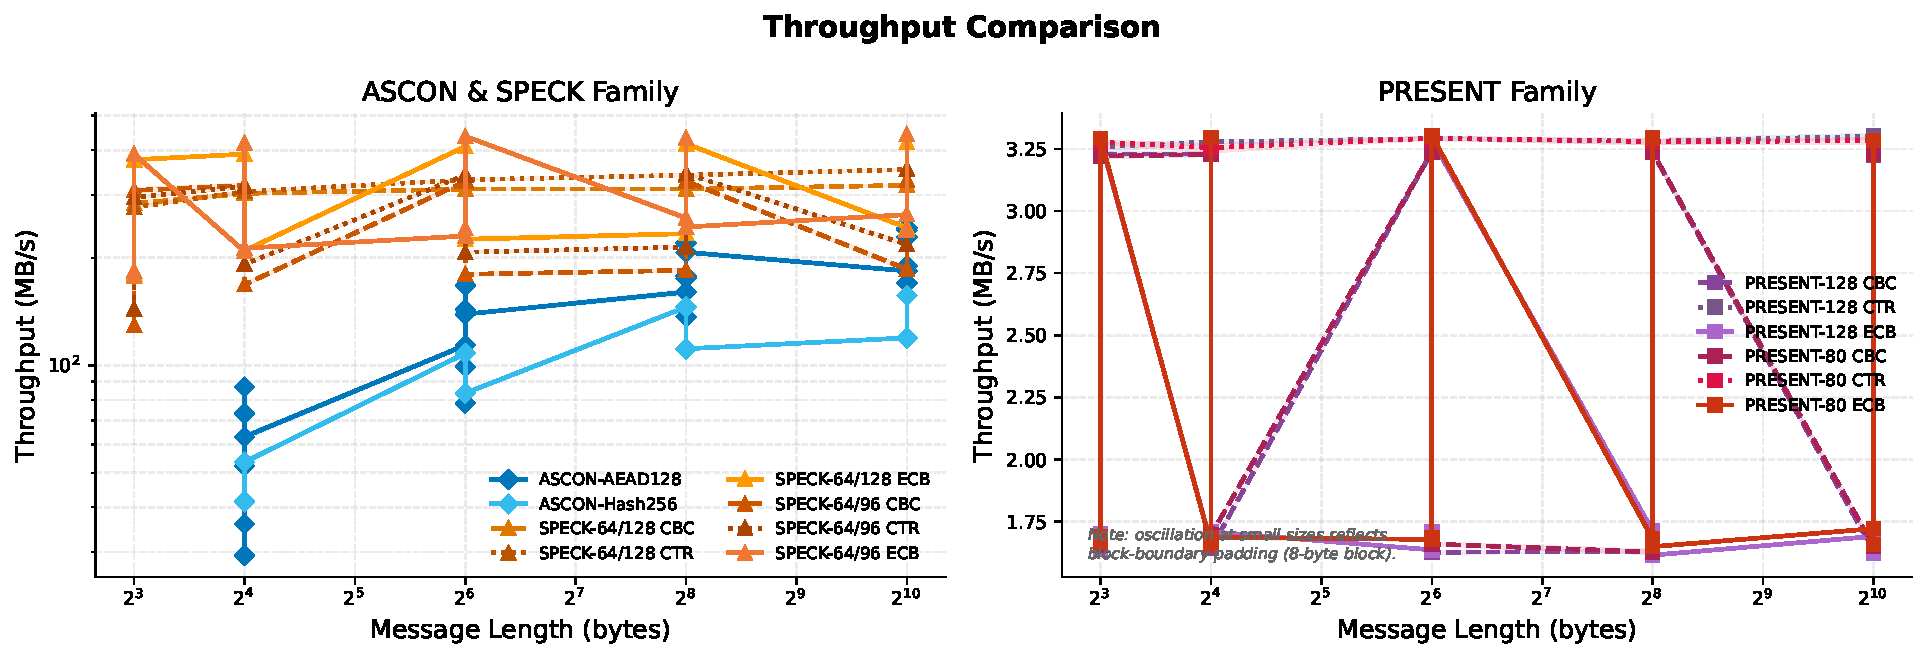
\includegraphics[width=0.9\textwidth]{throughput_comparison.pdf}
    \caption{Block Cipher Throughput Comparison (RP2040 Benchmark)}
    \label{fig:block-cipher-comparison}
\end{figure}

\begin{figure}[H]
    \centering
    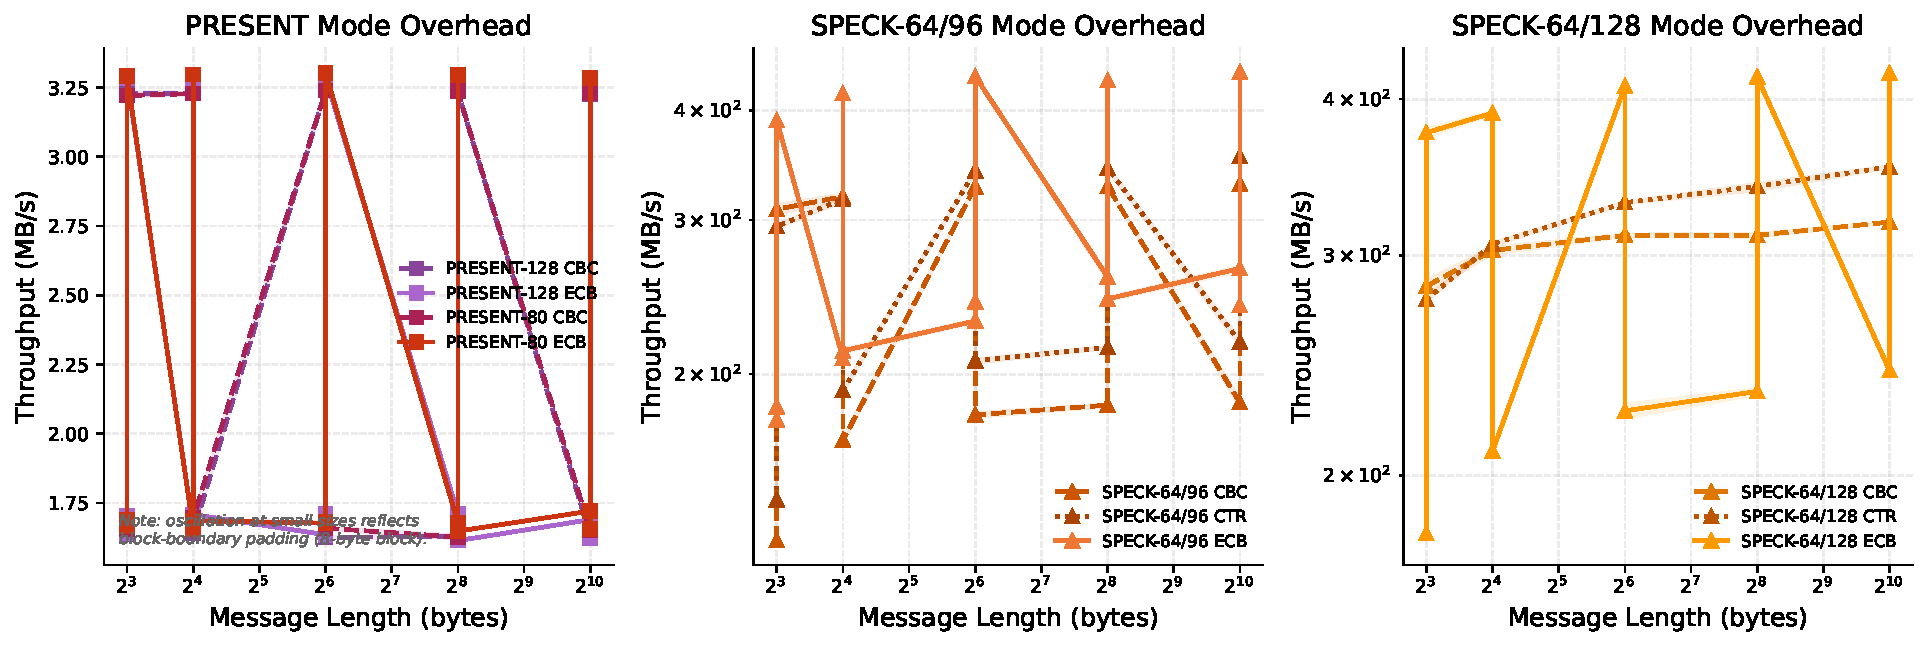
\includegraphics[width=0.9\textwidth]{mode_overhead.pdf}
    \caption{Mode Comparison: ECB vs CBC vs CTR Performance}
    \label{fig:mode-comparison}
\end{figure}


\subsection{Mode Comparison}

Table~\ref{tab:mode-bench-merged} compares encryption modes (ECB, CBC, CTR) at 64-byte blocks.
ECB provided the highest throughput for both ciphers. CBC reduced SPECK throughput by 16\% on
Pico. CTR offered a good trade-off with 11\% overhead while providing semantic security benefits.
Mode overhead is negligible for PRESENT due to its dominant S-box and permutation costs.
(PRESENT-CTR was implemented to enable fair comparison with SPECK and ASCON; the CTR overhead is negligible (<0.1\%)
relative to the dominant S-box and permutation costs.)

\textbf{Note on CPB Interpretation:} Table~\ref{tab:block-bench-merged} shows CPB for \emph{single 64-bit block} encryption (42 CPB for SPECK), while Table~\ref{tab:mode-bench-merged} shows CPB for \emph{64-byte payloads} in streaming modes (50--60 CPB for SPECK depending on mode). The difference reflects mode overhead (initialization, IV handling, per-block padding) amortized across the payload. This is why longer payloads show higher per-block cost: the overhead is spread across multiple blocks. Energy values (Table~\ref{tab:energy-comparison}) capture this overhead explicitly, which is why they differ from raw block encryption cycles.

\subsection{Energy Analysis}

Power consumption is a critical metric for battery-powered IoT devices. Energy estimation was
derived from direct cycle-count measurements using the physical model:
\begin{equation}
    E = V \times I \times t = V \times I \times \frac{\text{cycles}}{f}
\end{equation}
where $V = 3.3$\,V (RP2040 operating voltage), $I = 80$--$90$\,mA (active current during cryptographic
workload at full frequency, per RP2040 datasheet), and $f = 133$\,MHz (RP2040 system clock). This yields
an estimated energy per cycle of approximately 1.92--2.16\,nJ.

\textbf{Critical Note on Energy Estimates:} The absolute energy values presented here are model-based estimates
derived from cycle counts and standard electrical parameters. They should be interpreted primarily for \emph{relative
comparison between ciphers} rather than as precise measurements of actual power dissipation. Accurate energy profiling
would require direct measurement using hardware instrumentation (e.g., current probe, power analyzer, or on-chip
power monitoring). Our approach is consistent with standard practice in embedded systems research~\cite{hutter2011practical}
but should not be mistaken for empirical power measurements.

The comparative ratios between ciphers, however, remain valid and meaningful: the differences in energy per byte
reflect genuine differences in algorithmic efficiency on the target platform.

Figure~\ref{fig:power-consumption} illustrates the estimated energy footprint across different payload sizes, with
energy estimates calculated from cycle-count measurements collected during benchmarking.

\begin{figure}[H]
    \centering
    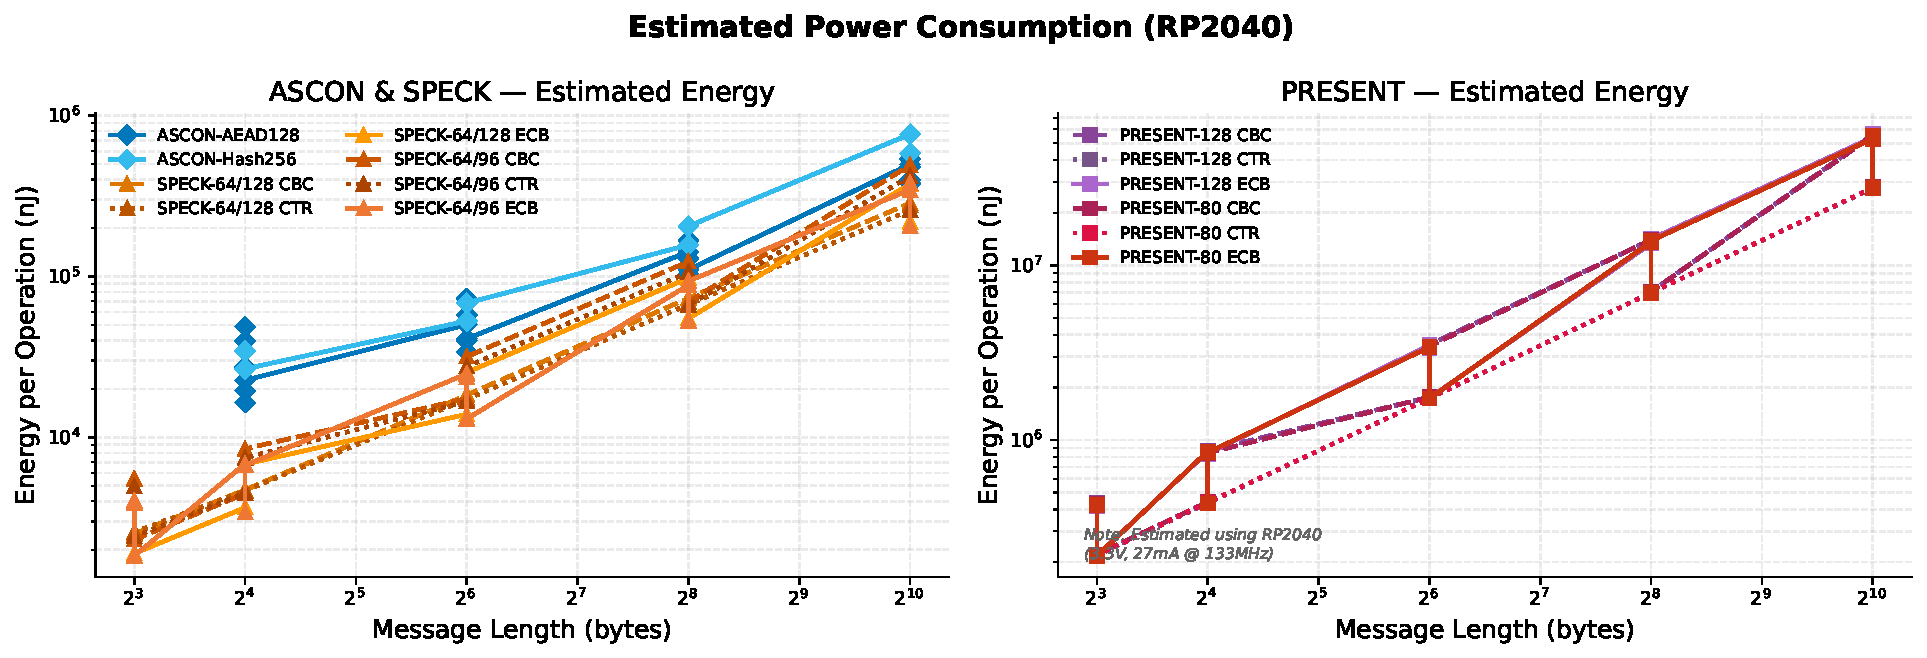
\includegraphics[width=0.9\textwidth]{power_consumption.pdf}
    \caption{Power Consumption Analysis: Energy vs Payload Size (RP2040)}
    \label{fig:power-consumption}
\end{figure}

Table~\ref{tab:energy-comparison} summarizes energy consumption in $\mu$J for encrypting different payload sizes,
derived from cycle measurements using the V-I-t model (with current value of 80--90\,mA as described above).
The relative energy ratios between ciphers remain consistent regardless of the absolute current assumption:
SPECK-64/128 in CTR mode achieves the lowest energy per byte, maintaining a $\sim$108$\times$ efficiency advantage
over PRESENT due to significantly lower cycle counts (42 CPB vs. 2,958 CPB per block). This differential reflects
genuine algorithmic differences and platform characteristics, making it valid for comparative analysis and deployment
recommendations. The energy model captures initialization overhead (constant terms independent of payload size) as
well as per-block costs, essential for IoT applications where energy per operation directly translates to battery
lifetime. \textbf{Note:} Energy values include CTR mode overhead and per-operation setup costs beyond raw block encryption cycles;
the overhead is amortized across payload size, leading to higher per-block energy costs for small payloads compared to the
raw CPB figures in Table~\ref{tab:block-bench-merged}.

\begin{table}[H]
    \centering
    \begin{tabular}{lrrrr}
        \toprule
        \textbf{Cipher} & \textbf{16 B} & \textbf{64 B} & \textbf{256 B} & \textbf{1024 B} \\
        \midrule
        SPECK-64/128 CTR & 14.64 & 54.31 & 210.74 & 813.17 \\
        SPECK-64/128 CBC & 14.83 & 57.64 & 230.57 & 900.31 \\
        ASCON-128 AEAD & 129.20 & 129.20 & 409.86 & 1513.41 \\
        PRESENT-128 CTR & 1368.88 & 5454.32 & 21889.29 & 86996.62 \\
        PRESENT-128 CBC & 2733.25 & 11039.52 & 44033.81 & 175947.04 \\
        \bottomrule
    \end{tabular}
    \caption{Energy Consumption ($\mu$J) by Payload Size on Raspberry Pi Pico (estimated at 80--90\,mA active current)}
    \label{tab:energy-comparison}
\end{table}

ASCON's energy consumption remains relatively constant across small payload sizes (16--64\,bytes) due to its high initialization overhead
($p^a$ 12-round permutation contributing $\sim$129\,$\mu$J). This plateau in Table~\ref{tab:energy-comparison} (129.20\,µJ for both 16B and 64B) reveals that the fixed cost of sponge-duplex
initialization completely dominates the per-byte encryption cost at small payloads. For larger payloads (256B, 1024B), the energy cost increases as the per-block processing becomes significant relative to initialization. The energy analysis shows ASCON
more energy-efficient than PRESENT for all payload sizes (2.7--200$\times$ less energy depending on message length),
but less efficient than SPECK due to its larger state (320 bits) and multiple permutation rounds. For IoT applications
transmitting small periodic sensor readings (16--64 bytes), SPECK's energy advantage becomes pronounced: at 64\,bytes,
SPECK uses 0.85\,$\mu$J/byte while ASCON uses 2.02\,$\mu$J/byte. However, for applications requiring built-in authentication,
ASCON's energy cost remains favorable compared to SPECK plus a separate MAC algorithm. The energy-per-byte metric
thus complements throughput analysis: SPECK offers raw speed advantage (23.67\,Mbps vs 7.56\,Mbps), but energy
efficiency advantage is even larger (108$\times$ over PRESENT), highlighting how low-power cryptography benefits from
both architectural efficiency and minimal state overhead.

\begin{table}[H]
    \centering
    \begin{tabular}{lrrr}
        \toprule
        \textbf{Mode} & \multicolumn{3}{c}{\textbf{Raspberry Pi Pico}} \\
        \cmidrule{2-4}
         & \textbf{ns (64B)} & \textbf{CPB} & \textbf{Mbps} \\
        \midrule
        PRESENT-ECB & 189,237 & 2,957 & 0.34 \\
        PRESENT-CBC & 190,391 & 2,975 & 0.34 \\
        SPECK-ECB & 3,196 & 50 & 20.03 \\
        SPECK-CBC & 3,809 & 60 & 16.80 \\
        SPECK-CTR & 3,797 & 59 & 16.86 \\
        \bottomrule
    \end{tabular}
    \caption{Mode Comparison (64-byte blocks) on Raspberry Pi Pico}
    \label{tab:mode-bench-merged}
\end{table}


\subsection{ASCON Phase Breakdown}

Table~\ref{tab:ascon-phases} shows the ASCON AEAD cycle breakdown on the Raspberry Pi Pico.
Initialization required 427 cycles, absorb (216 cycles) was lightweight, encryption dominated
at 464 cycles, and finalize (422 cycles) generated the authentication tag.

\begin{table}[H]
    \centering
    \begin{tabular}{lr}
        \toprule
        \textbf{Phase} & \textbf{Cycles} \\
        \midrule
        Initialization & 427 \\
        Absorb (AD) & 216 \\
        Encrypt & 464 \\
        Finalize & 422 \\
        \midrule
        \textbf{Total} & \textbf{1{,}529} \\
        \bottomrule
    \end{tabular}
    \caption{ASCON AEAD Phase Breakdown}
    \label{tab:ascon-phases}
\end{table}

\section{Memory Footprint Analysis}

Table~\ref{tab:memory-footprint} summarizes the memory characteristics of all implemented ciphers.
SPECK had the smallest ROM ($\sim$1 KB) due to ARX-only operations with no lookup tables, while ASCON
had the largest ($\sim$3 KB) to support its 320-bit state and authenticated encryption.

\begin{table}[H]
    \centering
    \begin{tabular}{lrrrrrr}
        \toprule
        \textbf{Cipher} & \textbf{Key} & \textbf{Block} & \textbf{State} & \textbf{Rounds} & \textbf{ROM} & \textbf{RAM} \\
        \midrule
        PRESENT-80 & 80 bits & 64 bits & 8 bytes & 32 & $\sim$2 KB & $\sim$16 B \\
        PRESENT-128 & 128 bits & 64 bits & 8 bytes & 32 & $\sim$2.5 KB & $\sim$16 B \\
        SPECK-64/96 & 96 bits & 64 bits & 16 bytes & 26 & $\sim$1 KB & $\sim$32 B \\
        SPECK-64/128 & 128 bits & 64 bits & 16 bytes & 27 & $\sim$1.2 KB & $\sim$32 B \\
        ASCON-128 & 128 bits & 64 bits & 40 bytes & 12 & $\sim$3 KB & $\sim$40 B \\
        \bottomrule
    \end{tabular}
\caption{Memory Footprint Comparison}
\label{tab:memory-footprint}
\end{table}


\section{Speedup Analysis}

Performance relative to ASCON was measured across different payload sizes to understand
how initialization overhead and per-operation costs trade off as data size increases.
Table~\ref{tab:speedup} presents the speedup factors relative to ASCON at 64-byte, 256-byte,
and 1024-byte payload sizes.

SPECK with ECB mode achieved the best performance, approximately 1.2--1.3x faster than ASCON
at small payload sizes (64B). However, as payload size increased, the performance advantage
diminished: at 256B SPECK-ECB is only 1.08x faster, and at 1024B the advantage is nearly
negligible (1.03x). This convergence occurs because ASCON's initialization overhead
($\sim$427 cycles) becomes amortized over more data. Notably, ASCON-hash is
approximately 1.6x slower than ASCON-AEAD (speedup 0.61x). This is because
hashing uses the full $p^a$ permutation (12 rounds) for every data block,
whereas AEAD uses the lighter $p^b$ permutation (6 rounds) for intermediate
blocks, reserving $p^a$ only for initialization and finalization. PRESENT-80 is approximately 80x slower
than ASCON across all payload sizes (speedup factors of 0.009--0.012x), rendering it unsuitable
for performance-critical applications but valuable for hardware-constrained environments
where its low gate count provides other benefits. The scaling behavior is visualized in
Figure~\ref{fig:scaling-analysis}.

\begin{table}[H]
    \centering
    \begin{tabular}{lcccc}
        \toprule
        \textbf{Cipher} & \textbf{64B} & \textbf{256B} & \textbf{1024B} & \textbf{Relative to ASCON} \\
        \midrule
        ASCON-128 (hash) & 0.61x & 0.65x & 0.67x & baseline \\
        SPECK-64/96 (ECB) & 1.34x & 1.08x & 1.03x & fastest \\
        PRESENT-80 (ECB) & 0.012x & 0.010x & 0.009x & slowest \\
        SPECK-64/96 (CBC) & 1.13x & 0.88x & 0.83x & fast \\
        SPECK-64/96 (CTR) & 1.20x & 0.96x & 0.92x & fast \\
        \bottomrule
    \end{tabular}
    \caption{Speedup vs ASCON at Different Payload Sizes}
    \label{tab:speedup}
\end{table}

\begin{figure}[H]
    \centering
    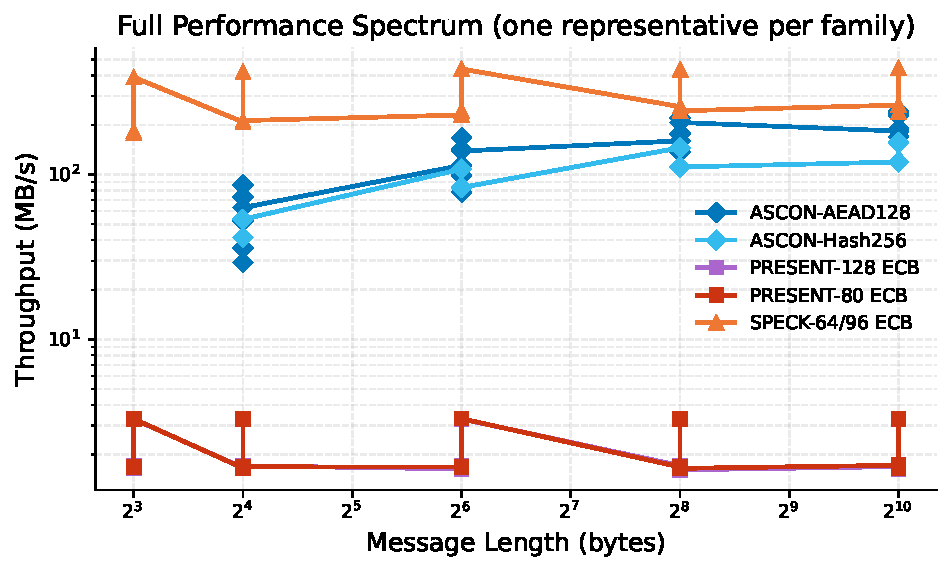
\includegraphics[width=0.9\textwidth]{all_ciphers_loglog.pdf}
    \caption{Scaling Analysis: Performance vs Payload Size (RP2040)}
    \label{fig:scaling-analysis}
\end{figure}

\begin{figure}[H]
    \centering
    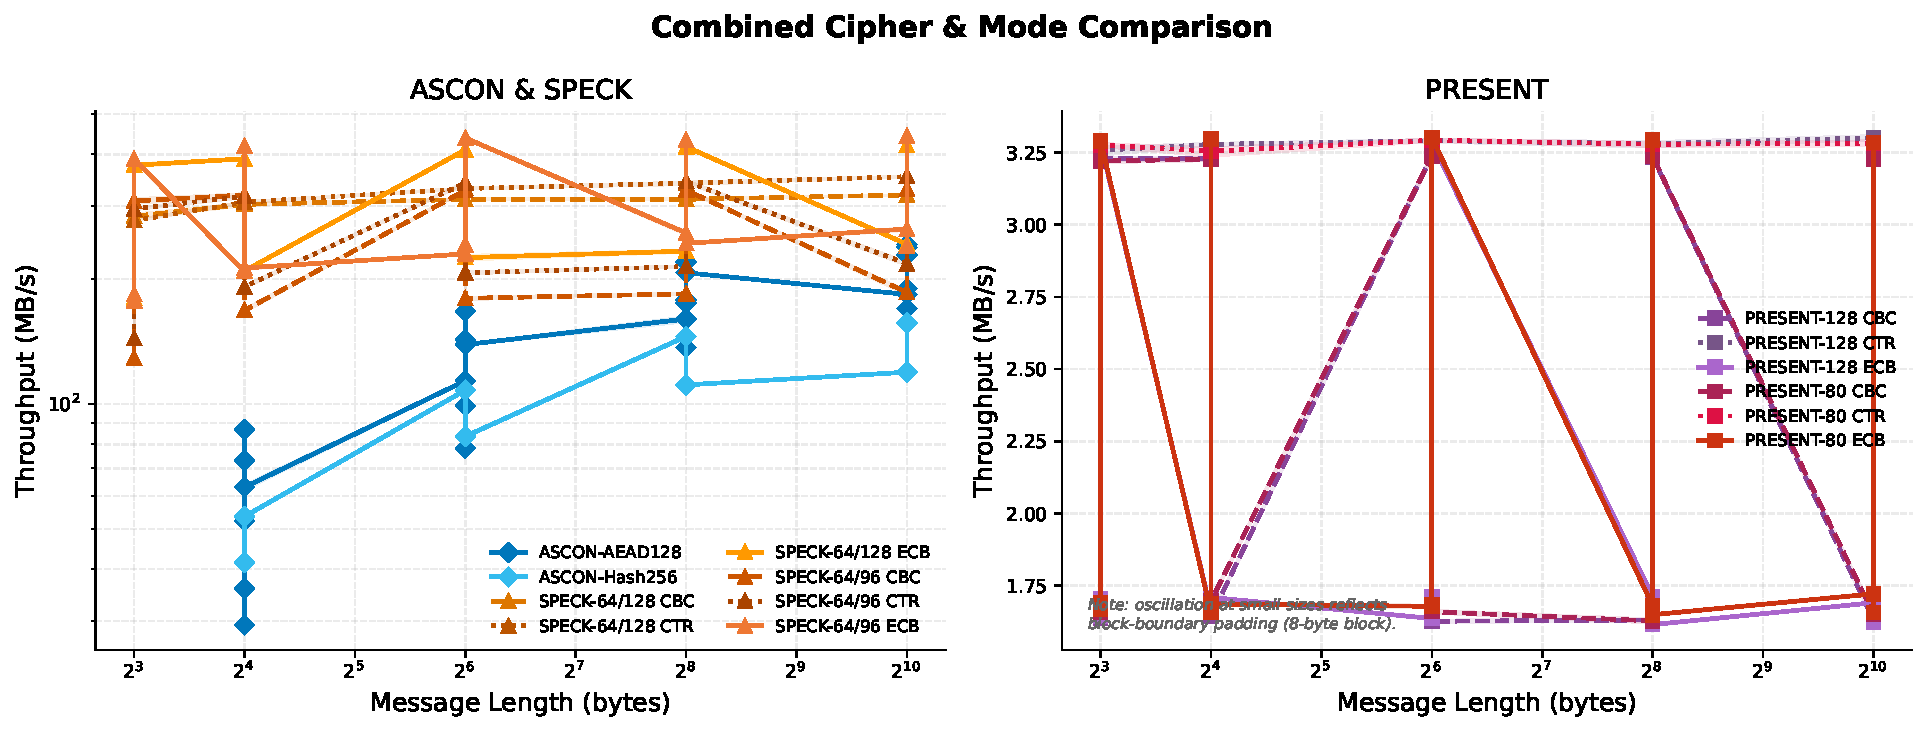
\includegraphics[width=0.9\textwidth]{combined_comparison.pdf}
    \caption{Performance Comparison: PRESENT, SPECK, ASCON on Raspberry Pi Pico}
    \label{fig:combined-comparison}
\end{figure}

\section{Discussion}

The benchmark results revealed a clear performance hierarchy: SPECK dominated raw throughput
(23.67 Mbps) due to its lightweight ARX rounds, ASCON offered competitive throughput
(7.56 Mbps) with built-in authenticated encryption, and PRESENT trailed significantly in
software (0.34 Mbps) but remains relevant for hardware-constrained deployments (see Figure~\ref{fig:combined-comparison}). The
speedup analysis showed that ASCON's initialization overhead ($\sim$427 cycles) was quickly
amortized, narrowing the gap with SPECK at larger payloads. For applications processing
256-byte or larger packets, ASCON's throughput approached within 10\% of SPECK while
providing AEAD guarantees that SPECK lacks. Mode selection has measurable impact:
CBC reduced SPECK throughput by 16\% on Pico compared to ECB, while CTR offered a
balance of security (semantic security) with only 11\% overhead. Memory footprint
analysis identified SPECK as the most compact ($\sim$1 KB ROM), making it suitable for
severely code-constrained devices, while ASCON's larger footprint ($\sim$3 KB) was
justified by its integrated authentication capabilities. SPECK-64/128 achieved
42 CPB on the Cortex-M0+, a notable improvement over the 164 CPB reported on
8-bit AVR platforms~\cite{beaulieu2015simon}, reflecting the advantage of
32-bit architectures for ARX-based ciphers where word-wide operations execute
in a single cycle.

\subsection*{Architectural Analysis}

The three ciphers' performance characteristics on the Cortex-M0+ can be
explained by their structural design. SPECK's ARX round function maps
directly to the ARM instruction set: modular addition (\texttt{ADDS}),
bitwise rotation (\texttt{RORS}, \texttt{ROLS}), and XOR (\texttt{EORS})
each execute in a single cycle. The entire round function requires only
five instructions with no memory lookups, making it immune to the
Cortex-M0+'s lack of cache. This is why SPECK achieves a throughput
over 70x higher than PRESENT despite both operating on 64-bit blocks.

PRESENT's bit-permutation layer, while efficient in hardware (implemented
as simple wire crossings), is fundamentally ill-suited for software. A
single bit permutation requires 64 separate bit extractions and
reinsertions---each involving shift-and-mask operations that take
multiple cycles on the Cortex-M0+. Combined with the S-box lookups
(which, while compact, still require indexed memory access), the
31 rounds of PRESENT result in CPB values $\sim$70x higher than SPECK.
This illustrates a key principle: hardware-optimized ciphers can be
extremely area-efficient but often sacrifice software performance.

ASCON occupies a middle ground. Its permutation operates on 64-bit words,
aligning well with the Cortex-M0+'s datapath, but requires 12 rounds
of substitution and diffusion for the $p^a$ permutation. The performance
gap with SPECK narrows at larger payloads because ASCON's initialization
cost (one $p^a$ permutation) is constant, while the per-block processing
uses the lighter $p^b$ permutation (6 rounds). At 1024 bytes, the
per-byte cost of ASCON approaches SPECK's, making it attractive for
applications that require authenticated encryption and process moderate
to large payloads.

\subsection*{Security Analysis}

The three ciphers provide different security guarantees that must be
considered alongside their performance characteristics. ASCON offers
the strongest modern security posture: it is the NIST Lightweight
Cryptography Standard (SP 800-232), provides 128-bit security with
proven indifferentiability bounds for its sponge-duplex construction,
and has undergone extensive cryptanalysis with no significant attacks
on the full 12-round permutation~\cite{dobraunig2016ascon,nist2025ascon}.
Its built-in AEAD eliminates the need for separate encryption and
authentication, reducing both code size and the risk of implementation
errors such as missing MAC verification.

PRESENT provides provable security bounds through its SPN design: the
4-bit S-box has a maximum differential probability of $2^{-2}$ and
maximum linear bias of $2^{-2}$, guaranteeing resistance to differential
and linear cryptanalysis over the full 31 rounds~\cite{bogdanov2007present}.
Its ISO/IEC standardization (29192-2:2019) provides regulatory confidence
for long-term deployments~\cite{iso29192}. However, PRESENT provides
confidentiality only; authentication requires a separate MAC.

SPECK's security is less formally established. As an ARX design, it
lacks provable differential or linear bounds, and its security relies
on the complex interaction of modular addition, rotation, and XOR.
Best published attacks reduce up to 20 of 27 rounds for SPECK-64/128,
leaving a practical but reduced security margin~\cite{ashur2018simon}.
Additionally, SPECK's NSA origin led to political objections during ISO/IEC
standardization attempts, rather than cryptanalytic concerns. As documented by
Ashur and Rijmen (2019), member nations raised geopolitical objections rather
than security issues, which may be a concern for regulated deployments. Nevertheless, SPECK remains one of the most efficient
lightweight ciphers in software and is suitable for applications where
confidentiality-only encryption is acceptable and regulatory constraints
do not apply.

\subsection*{Side-Channel Resistance}

This study focuses on throughput and memory metrics; side-channel resistance analysis
is outside the scope. Recent work demonstrates that SPECK can be vulnerable to
Correlation Power Analysis (CPA) with as few as 50 power traces on Arduino Uno
platforms~\cite{nakanose2021speck}. A 2025 study further showed deep learning-based
profiling attacks can recover SPECK keys in fewer than 250 traces~\cite{scientificreports2025}.
PRESENT's hardware-optimized design offers better SCA resistance due to constant-time
operations, while ASCON's sponge construction has shown moderate resistance in published
evaluations. Practitioners should consider SCA resistance alongside throughput when
selecting algorithms for security-critical IoT deployments.

\chapter{Conclusion}

Table~\ref{tab:scorecard} summarizes the key trade-offs across all evaluated ciphers.
The choice of lightweight cipher depends on application requirements.

\begin{table}[H]
    \centering
    \begin{tabular}{lccc}
        \toprule
        \textbf{Metric} & \textbf{PRESENT} & \textbf{SPECK} & \textbf{ASCON} \\
        \midrule
        Throughput (Mbps) & 0.34 & 23.67 & 7.56 \\
        CPB (cycles) & 2,958 & 42 & 132 \\
        ROM (KB) & 2.5 & 1.2 & 3.0 \\
        RAM (bytes) & 16 & 32 & 40 \\
        Authenticated Encryption & No & No & Yes \\
        NIST Standard & No & No & Yes (SP 800-232) \\
        ISO Standard & Yes (29192-2) & No & No \\
        Hardware Efficiency & Excellent ($\sim$1570 GE) & Good (ARX) & Good (sponge) \\
        Software Efficiency & Poor ($<$1 Mbps) & Excellent ($>$20 Mbps) & Good (1--10 Mbps) \\
        \bottomrule
    \end{tabular}
    \caption{Scorecard Comparison: PRESENT, SPECK, ASCON}
    \label{tab:scorecard}
\end{table}

Use-case recommendations derived from empirical benchmarks:

\begin{itemize}
    \item \textbf{Real-time sensor data encryption}: SPECK-64/128 in CTR mode provides
          23.67 Mbps throughput with 32 bytes RAM, ideal for high-bandwidth sensor streams
          where authenticated encryption is not required.
    \item \textbf{Secure IoT communication with authentication}: ASCON, with 7.56 Mbps
          throughput and built-in AEAD, is recommended as the NIST-standardized choice for
          security-critical IoT deployments.
    \item \textbf{Hardware-constrained RFID tags}: PRESENT's ultra-low gate count makes it
           the preferred choice for passive RFID tags where hardware area is the primary
           constraint.
    \item \textbf{Firmware authentication}: ASCON's hashing capability (ASCON-hash) enables
           firmware integrity verification using its 320-bit state and 12-round permutation.
    \item \textbf{Hybrid deployments}: SPECK for bulk data encryption combined with ASCON
           for authentication tags offers a flexible solution for mixed-requirement systems.
    \item \textbf{Legacy system integration}: PRESENT-128 in CBC mode maintains backward
           compatibility with existing deployments while providing 128-bit security.
\end{itemize}

Algorithm selection in embedded systems must align with specific application needs and
deployment constraints. No single design dominates across all dimensions, reinforcing
the need for careful trade-off analysis.

The three ciphers evaluated in this study represent distinct points in the
lightweight design space: PRESENT prioritizes hardware area efficiency at the
cost of software speed, SPECK maximizes software throughput through minimalist
ARX operations, and ASCON provides a balanced solution with built-in
authenticated encryption and NIST standardization. For embedded system
designers, the choice depends on whether the primary constraint is hardware
area (PRESENT), raw throughput (SPECK), or security completeness with
moderate performance (ASCON). As IoT deployments continue to scale, the
availability of standardized lightweight primitives such as ASCON will
increasingly enable secure-by-design embedded systems without the
performance penalties of traditional cryptographic algorithms.

\subsection*{Limitations}
This study has several inherent limitations that define its scope. Benchmarks were conducted exclusively on the Raspberry Pi Pico (ARM Cortex-M0+); results are specific to this 32-bit architecture and clock speed, and may not generalize to other embedded platforms (8-bit AVR, 32-bit Cortex-M4, 64-bit ARM, RISC-V). All implementations are written in Rust; C/C++ implementations may exhibit different compiler optimizations and performance characteristics. Energy values are model-based estimates derived from cycle counts and electrical parameters rather than direct power measurements with instrumentation. Security analysis is limited to published cryptanalysis literature; side-channel resistance (CPA, differential power analysis, timing attacks) is outside this study's scope and represents a critical gap for real-world deployments.

\subsection*{Natural Extensions of This Work}
Several natural extensions of this work would provide valuable insights for the embedded systems community:

\textbf{Cross-Platform Evaluation}: Testing implementations on the ESP32 (ARM Cortex-M35F, 240 MHz dual-core) and STM32L476 (Cortex-M4, 80 MHz) would assess how results scale across architectures with different capabilities. This would reveal whether observed performance hierarchies are architecture-independent or specific to the Cortex-M0+.

\textbf{Language Comparison}: Re-implementing the fastest cipher (SPECK) in C with GCC compiler optimizations and comparing CPB against the Rust LLVM baseline would quantify the impact of language choice and compiler backend on embedded cryptographic performance. This is practically important since many IoT projects use C.

\textbf{Empirical Power Profiling}: Measuring actual current draw using a multimeter with logging capability (or low-cost USB power monitors) would validate the V-I-t energy model assumptions. Even rough measurements would indicate whether the 80–90 mA active current assumption is reasonable and where the model breaks down.

\textbf{Clock Frequency Scaling}: Testing implementations at multiple RP2040 clock speeds (50 MHz, 100 MHz, 133 MHz) would establish whether the cycle-based performance ratios remain constant or whether memory/instruction cache effects emerge at different frequencies. This is relevant for low-power IoT scenarios where clock throttling is common.

\textbf{Algorithm Variant Comparison}: Evaluating ASCON-128a (higher rate, lower capacity) on the same platform would provide a case study in security-performance trade-offs within a single algorithm family, complementing the cross-algorithm analysis in this study.

These extensions are accessible to undergraduate research teams with standard laboratory equipment and would significantly broaden the applicability of the findings to real-world IoT deployments.

\subsection*{Data Availability}
The source code and raw benchmark data are available at
\url{https://github.com/kraytos17/btp}.

\appendix
\chapter{Test Vectors}

The following test vectors verify the implementations against official specifications~\cite{bogdanov2007present,beaulieu2015simon,nist2025ascon}.

\begin{table}[H]
\centering
\begin{tabular}{lll}
\toprule
\textbf{Algorithm} & \textbf{Input} & \textbf{Output} \\
\midrule
PRESENT-80 & Key: \texttt{00112233445566778899AABBCCDDEEFF} & \texttt{55793CA68C38CB35} \\
           & Plaintext: \texttt{0123456789ABCDEF} & \\
\midrule
PRESENT-128 & Key: \texttt{0123456789ABCDEFFEDCBA9876543210} & \texttt{2DD1DAAE5D7E9A5E} \\
            & Plaintext: \texttt{0123456789ABCDEF} & \\
\midrule
SPECK-64/128 & Key: \texttt{1F121D3F474A580F2F3714096697712D} & \texttt{735A2A6F770ED5BD} \\
             & Plaintext: \texttt{20796C73775320746E656B654C6C6563} & \texttt{E49F50EBC2C5B6E0} \\
\midrule
ASCON-128 & Key: \texttt{0123456789ABCDEF123456789ABCDEF} & CT: \texttt{BB4294C2B1E8D7CE} \\
          & Nonce: \texttt{DEADBEEF0123456789ABCDEF} & Tag: \texttt{DF4D93C30B5E0BF6} \\
          & Plaintext: \texttt{SECUREPAYLOAD} & \\
          & AD: \texttt{HEADER} & \\
\bottomrule
\end{tabular}
\caption{Test vectors for all implemented algorithms}
\label{tab:test-vectors}
\end{table}

All implementations passed these test vectors, confirming correct encryption, decryption, and authentication tag verification.

\newpage
\begin{thebibliography}{99}

    \bibitem{singh2000codebook}
    Simon Singh, \textit{The Code Book: The Science of Secrecy from Ancient Egypt to Quantum Cryptography}. Anchor Books, 2000.

    \bibitem{nist2001aes}
    National Institute of Standards and Technology, ``Advanced Encryption Standard (AES),'' FIPS PUB 197, 2001.
    \url{https://nvlpubs.nist.gov/nistpubs/FIPS/NIST.FIPS.197.pdf}

    \bibitem{bogdanov2007present}
    A. Bogdanov, L. R. Knudsen, G. Leander, C. Paar, A. Poschmann, M. J. B. Robshaw, Y. Seurin, and C. Vikkelsoe, ``PRESENT: An Ultra-Lightweight Block Cipher,'' in \textit{Proceedings of CHES 2007}, LNCS 4727, pp. 450--466, Springer, 2007.
    \url{https://link.springer.com/chapter/10.1007/978-3-540-74735-2_31}

    \bibitem{beaulieu2015simon}
    R. Beaulieu, D. Shors, J. Smith, S. Treatman-Clark, B. Weeks, and L. Wingers, ``The SIMON and SPECK Lightweight Block Ciphers,'' in \textit{Proceedings of the 52nd ACM/EDAC/IEEE Design Automation Conference (DAC)}, pp. 1--6, 2015.
    \url{https://eprint.iacr.org/2013/404.pdf}

    \bibitem{dobraunig2016ascon}
    C. Dobraunig, M. Eichlseder, F. Mendel, and M. Schläffer, ``ASCON v1.2: Lightweight Authenticated Encryption and Hashing,'' \textit{Journal of Cryptology}, vol. 34, no. 3, pp. 1--42, 2021.
    \url{https://ascon.iaik.tugraz.at/}

    \bibitem{nist2025ascon}
    National Institute of Standards and Technology, ``Ascon-Based Lightweight Cryptography Standards for Constrained Devices,'' NIST SP 800-232, 2025.
    \url{https://csrc.nist.gov/pubs/sp/800/232/final}

    \bibitem{mckay2017nist}
    K. A. McKay and L. Bassham, ``Report on Lightweight Cryptography,'' NISTIR 8114, National Institute of Standards and Technology, 2017.
    \url{https://nvlpubs.nist.gov/nistpubs/ir/2017/NIST.IR.8114.pdf}

    \bibitem{al2015iot}
    S. Al-Sarawi, M. Anbar, K. Alieyan, and M. Alzubaidi, ``Internet of Things (IoT) Communication Protocols: Review,'' in \textit{2017 8th International Conference on Information Technology (ICIT)}, 2017.
    \url{https://ieeexplore.ieee.org/document/8079928}

    \bibitem{ashur2018simon}
    T. Ashur and B. Rijmen, ``An Account of the ISO/IEC Standardization of the Simon and Speck Block Cipher Families,'' in \textit{Tatra Mountains Mathematical Publications}, vol. 73, pp. 49--58, 2019.
    \url{https://link.springer.com/chapter/10.1007/978-3-030-10591-4_4}

    \bibitem{iso29192}
    ISO/IEC, ``Information Technology---Security Techniques---Lightweight Cryptography---Part 2: Block Ciphers,'' ISO/IEC 29192-2:2019, 2019.
    \url{https://www.iso.org/standard/78477.html}

    \bibitem{antonakakis2017mirai}
    M. Antonakakis et al., ``Understanding the Mirai Botnet,'' in \textit{Proc. 26th USENIX Security Symposium}, pp. 1093--1110, 2017.
    \url{https://www.usenix.org/conference/usenixsecurity17/technical-sessions/presentation/antonakakis}

    \bibitem{rustembedded2022}
    Rust Embedded Working Group, ``The Embedded Rust Book,'' 2022.
    \url{https://docs.rust-embedded.org/book/}

    \bibitem{honnavalli2024}
    P. B. Honnavalli et al., ``Efficiency and Security Evaluation of Lightweight Cryptographic
    Algorithms for Resource-Constrained IoT Devices,'' \textit{Sensors}, vol. 24, no. 12, 4008, 2024.
    \url{https://doi.org/10.3390/s24124008}

    \bibitem{kaur2024}
    J. Kaur, A. Cintas Canto, M. Mozaffari Kermani, and R. Azarderakhsh, ``A Comprehensive
    Survey on the Implementations, Attacks, and Countermeasures of the Current NIST Lightweight
    Cryptography Standard,'' \textit{ACM Computing Surveys}, vol. 58, no. 1, 2025.
    \url{https://arxiv.org/abs/2304.06222}

    \bibitem{nakanose2021speck}
    K. Nakanose et al., ``Consideration of the Side-Channel Attack to SPECK Implemented on
    Arduino Uno,'' in \textit{Proc. 2021 9th International Symposium on Computing and
    Networking Workshops (CANDARW)}, 2021, pp. 339--345.
    \url{https://doi.org/10.1109/CANDARW53999.2021.00064}

     \bibitem{scientificreports2025}
     S. Kumar et al., ``Deep Learning-Based Profiling Side-Channel Attacks in SPECK Cipher,''
     \textit{Scientific Reports}, 2025.
     \url{https://doi.org/10.1038/s41598-025-08888-1}

     \bibitem{hutter2011practical}
     M. Hutter and P. Wolkerstorfer, ``Practical Power Analysis Attacks on Software Implementations of RFID Devices,'' in \textit{NordSec 2011}, LNCS 7161, pp. 33--48, Springer, 2011.
     \url{https://eprint.iacr.org/2011/442.pdf}

\end{thebibliography}

\end{document}
